\documentclass[a4paper]{article}
% \usepackage[utf8]{inputenc}
\usepackage{fontspec}
\usepackage{xcolor}
\setmainfont{TeX Gyre Pagella}

\usepackage[margin=0cm]{geometry}
\usepackage{tikz}
\usetikzlibrary {shapes.geometric}


\begin{document}
\pagestyle{empty}
\parindent 0pt
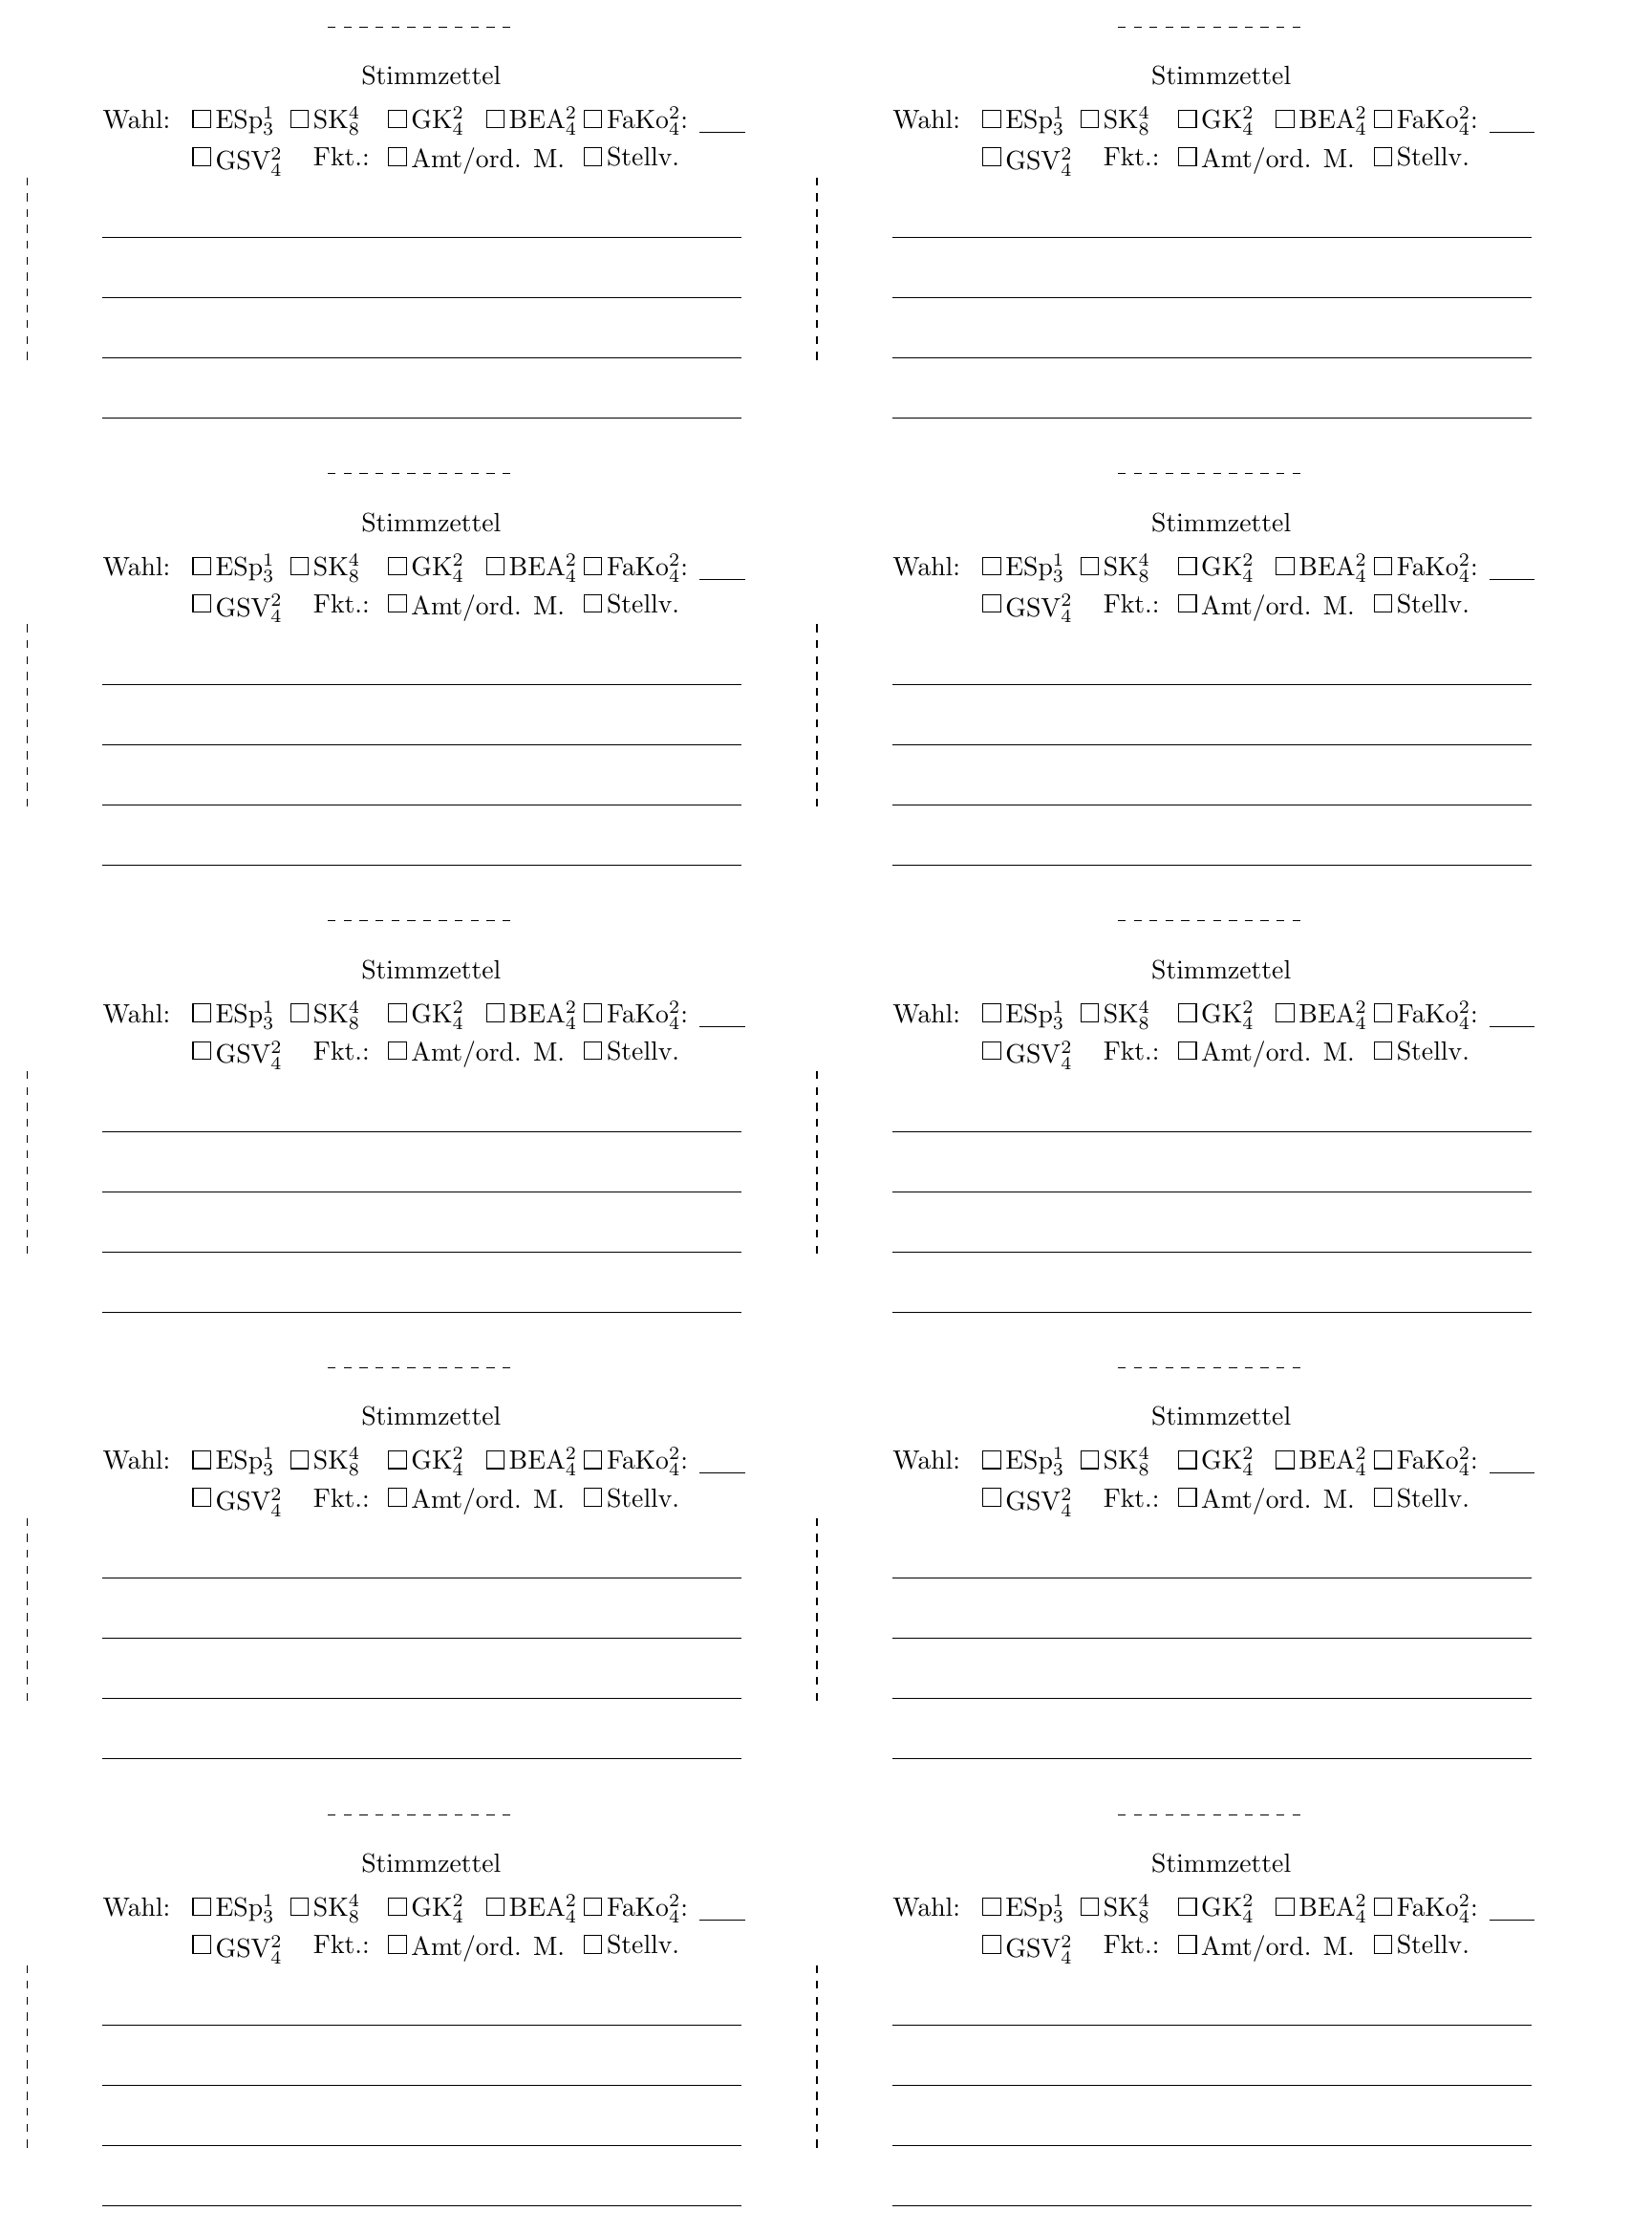
\begin{tikzpicture}[x=1mm,y=-1mm,
every node/.style={anchor=north west},
lab/.style={anchor=north west,inner sep=0mm},
num/.style={circle,anchor=north west,inner sep=0.5mm}
]
\foreach \i in {0mm,105mm}
\foreach \j in {0mm,59.4mm,118.8mm,178.2mm,237.6mm}
{
\begin{scope}[xshift=\i,yshift=\j]
  \begin{scope}[yshift=-4mm]
  \path (0,0) node [text width=105mm,align=center,
  anchor=north west] {Stimmzettel}
       (10,7) node [lab] {Wahl:} 
       (38,12) node [lab] {Fkt.:} ;
  
  \foreach \labr/\labrb in {6.6/7}
  \path
  (22,\labrb) node[draw] {}
  (25,\labr) node[lab] {ESp$^1_3$}
  (35,\labrb) node[draw] {}
  (38,\labr) node[lab] {SK$^4_8$}
  (48,\labrb) node[draw] {}
  (51,\labr) node[lab] {GK$^2_4$}
  (61,\labrb) node[draw] {}
  (64,\labr) node[lab] {BEA$^2_4$}
  (74,\labrb) node[draw] {}
  (77,\labr) node[lab] {FaKo$^2_4$: \underline{\hspace{6mm}}}
  ; 
  \foreach \labr in {12}
  \path
  (22,\labr) node[draw] {}
  (25,\labr) node[lab] {GSV$^2_4$}
  (48,\labr) node[draw] {}
  (51,\labr) node[lab] {Amt/ord. M.}
  (74,\labr) node[draw] {}
  (77,\labr) node[lab] {Stellv.}
  ; 
  \end{scope}
  \begin{scope}[yshift=-28mm]
  \draw (10,0)  -- (95,0) ;
%   \path (12,-5) node[draw,num] {1};
%   \path (90,-5) node[draw,num] {5};
  \draw (10,8)  -- (95,8) ;
%   \path (12,3) node[draw,num] {2};
%   \path (90,3) node[draw,num] {6};
  \draw (10,16) -- (95,16);
%   \path (12,11) node[draw,num] {3};
%   \path (90,11) node[draw,num] {7};
  \draw (10,24) -- (95,24);
%   \path (12,19) node[draw,num] {4};
%   \path (90,19) node[draw,num] {8};
  \end{scope}
  \draw[dashed,thin] (40,0) -- (65,0);
%   \draw[dotted,thin] (40,59.4) -- (65,59.4);
  \draw[dashed,thin] (0,20) -- (0,45);
%   \draw[dotted,thin] (105,20) -- (105,45);
\end{scope}
};
%   \draw (\i,\j) node[draw=none,text width=105mm] {
%   Wahlzettel  jksjkfjkdjf slfkdflkds sakdjksajdk kjsdkjsak 
%   ksjdksjdk kjdkjskd kjdkjs ksdkskdm ksjdkjskdj
%   };
\end{tikzpicture}
\end{document}
 
